\documentclass[10pt]{beamer}
 
\usepackage{macros-beamer}

\usepackage[utf8]{inputenc}

\usepackage{tikz-cd}

\usetikzlibrary{decorations.pathmorphing}
\usetikzlibrary{decorations.markings}
\tikzset{
	% >=stealth', %%  Uncomment for more conventional arrows
    vector/.style={decorate, decoration={snake}, draw},
	provector/.style={decorate, decoration={snake,amplitude=2.5pt}, draw},
	antivector/.style={decorate, decoration={snake,amplitude=-2.5pt}, draw},
    fermion/.style={draw=black, postaction={decorate},
        decoration={markings,mark=at position .55 with {\arrow[draw=black]{>}}}},
    fermionbar/.style={draw=black, postaction={decorate},
        decoration={markings,mark=at position .55 with {\arrow[draw=black]{<}}}},
    fermionnoarrow/.style={draw=black},
    gluon/.style={decorate, draw=black,
        decoration={coil,amplitude=4pt, segment length=5pt}},
    scalar/.style={dashed,draw=black, postaction={decorate},
        decoration={markings,mark=at position .55 with {\arrow[draw=black]{>}}}},
    scalarbar/.style={dashed,draw=black, postaction={decorate},
        dwecoration={markings,mark=at position .55 with {\arrow[draw=black]{<}}}},
    scalarnoarrow/.style={dashed,draw=black},
    electron/.style={draw=black, postaction={decorate},
        decoration={markings,mark=at position .55 with {\arrow[draw=black]{>}}}},
	bigvector/.style={decorate, decoration={snake,amplitude=4pt}, draw},
}

\newcommand{\vin}{\rotatebox[origin=c]{-90}{$\in$}}
 
 \setbeamertemplate{footline}[frame number]
 
%Information to be included in the title page:
\title{Higher Kac-Moody algebras}
\author{Brian Williams}
\institute{Northeastern University}
\date{June 13, 2018}

\begin{document}

\frame{\titlepage}

\begin{frame}
\frametitle{Outline of this talk}
\begin{enumerate}
\item Higher dimensional Kac-Moody algebras and sphere algebras.
\item Boundary conditions for gauge theories.
\item An approach to AdS/CFT.
\end{enumerate}
\end{frame}

\begin{frame}
\frametitle{Current algebras}

\begin{itemize}
\item Symmetries of (perturbative) quantum field theories described by (dg) Lie algebras. 
Locality $\rightsquigarrow$ sheaves/cosheaves of Lie algebras.
\item Throughout this talk $X$ is a complex manifold. 
We are interested in {\em holomorphic} field theories on $X$.
\item Holomorphic gauge symmetries by a Lie algebra $\fg$ leads to sheaf of Lie algebras $\sO^{hol}_X \tensor \fg$. 
Resolve by vector bundles and use sheaf of dg Lie algebras $$\Omega^{0,*}_X \tensor \fg$$ equipped with $\dbar$. 
Also have its cosheaf version $\Omega^{0,*}_{X,c} \tensor \fg$. 
\item Geometrically, $T_{\rm triv} {\rm Bun}_G(X)[-1] \simeq \Omega^{0,*}(X) \tensor \fg$. 
\item {\em Local Lie algebras}. Sections of graded vector bundles equipped with differential and bi-differential operators defining the differential and Lie bracket at the level of (co)sheaves. 
\item Costello-Gwilliam: observables of a QFT form a {\em factorization algebra}. 
Can also model symmetries by factorization algebras. 
\end{itemize}

\end{frame}

\begin{frame}
\frametitle{Enveloping algebras}

For any open set $U \subset X$ consider the Chevalley-Eilenberg cochain complex (computing Lie algebra {\em homology})
\ben
\clieu_*(\Omega^{0,*}_c(U) \tensor \fg) = \left(\Sym\left(\Omega^{0,*}_c(U) \tensor \fg[1]\right), \dbar + \d_\fg\right) .
\een
As we vary the open sets $U \subset X$ these complexes combine to form a factorization algebra, called the {\em factorization enveloping algebra} of $\Omega^{0,*}_X \tensor \fg$ that we denote $U^{fact}(\Omega^{0,*}_X \tensor \fg)$. 

When $\dim_\CC = 1$ this recovers the chiral envelope of Beilinson-Drinfeld.
In fact, when placed on $X = \CC$, Costello-Gwilliam show the following.

\begin{prop}[Costello-Gwilliam]
The factorization algebra $U^{fact}(\Omega^{0,*} \tensor \fg)$ on $X = \CC$ determines a vertex algebra with underlying vector space 
\ben
\Sym (\sO^{hol} (D)^\vee \tensor \fg) \cong \Sym(z^{-1} \fg[z^{-1}]) ,
\een
where $D\subset \CC$ is the unit disk, that is isomorphic to the {\bf Kac-Moody vertex algebra} of central charge zero.
\end{prop}

%Recall, the ``fields" of the Kac-Moody consist of $X (z) = \sum_{n} X_n z^n$ where $X \in \fg$.
%The OPE is
%\ben
%X(z_1) Y(z_2) \sim \frac{[X,Y]}{z_1-z_2} .
%\een

\end{frame}

\begin{frame}
\frametitle{Currents}

The {\em currents} of a QFT are those operators supported on codimension one submanifolds; for instance $S^{2d-1} \subset \CC^d$. 

When $d=1$ we have $\CC^\times = S^1 \times \RR_{>0}$ and can obtain a factorization algebra on $\RR_{>0}$ by pushing forward one on $\CC^\times$ along the projection map $\pi : S^1 \times \RR_{>0} \to \RR_{>0}$.
``Reduction along $S^1$". 

\ben
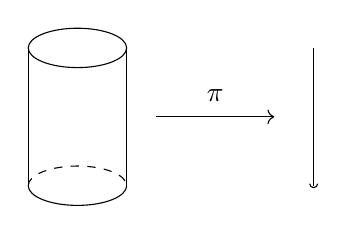
\begin{tikzpicture}[scale=0.5]
\draw (0,0) ellipse (1.25 and 0.5);
\draw (-1.25,0) -- (-1.25,-3.5);
\draw (-1.25,-3.5) arc (180:360:1.25 and 0.5);
\draw [dashed] (-1.25,-3.5) arc (180:360:1.25 and -0.5);
\draw (1.25,-3.5) -- (1.25,0);  
%\fill [gray,opacity=0.5] (-1.25,0) -- (-1.25,-3.5) arc (180:360:1.25 and 0.5) -- (1.25,0) arc (0:180:1.25 and -0.5);

\draw[->] (2, -1.75) -- (5,-1.75) ;

\node (pi) at (3.5, -1.2) {$\pi$};
\draw (6, -3.5) -- (6, 0);
\draw (5.9,-3.45) arc(180:360:0.1cm); 

\end{tikzpicture}
\een

Take the factorization enveloping algebra $U^{fact}(\Omega^{0,*} \tensor \fg)$ on $\CC^\times$.
The pushforward along $\pi$ is a locally constant factorization algebra on $\RR_{>0}$ which is equivalent, as an associative algebra, to 
\ben
U (\fg[z,z^{-1}]) = U({\rm algebraic\;loops\;in\;} \fg) .
\een

\end{frame}

\begin{frame}
\frametitle{Higher dimensions}

We now consider $U^{fact}(\Omega^{0,*}\tensor \fg)$ on higher dimensional affine space $\CC^d$, or its puncture $\CC^{d} \setminus 0$. 

For currents, we view $\CC^d \setminus 0 = S^{2d-1} \times \RR_{>0}$ and reduce along
\ben
\pi : S^{2d-1} \times \RR_{>0} \to \RR_{>0} .
\een
Take a algebraic Dolbeault model for $\CC^d \setminus 0$ $\rightsquigarrow$ commutative dg algebra $A_d$ concentrated in degrees $0,\ldots,d-1$ modeling punctured affine space $\AA^d \setminus 0$.  

\begin{prop}[W.] 
The pushforward of $U^{fact}(\Omega^{0,*}\tensor \fg)$ along $\pi$ is a locally constant factorization algebra. 
It is equivalent, as a dg associative algebra, to
\ben
U(A_d \tensor \fg) .
\een
\end{prop}

When $d=1$ this recovers the ordinary loop algebras.
In general, we get ``sphere algebras" which have interesting derived directions.

\end{frame}

\begin{frame}
\frametitle{Example: $d = 2$}

When $d=2$ one has
\ben
H^*(A_2) = \CC[z_1,z_2] \oplus z_{1}^{-1} z_2^{-1} \CC[z_1^{-1},z_2^{-1}][-1] .
\een
This is a commutative graded algebra.
In degree zero have the commutative algebra $\CC[z_1,z_2]$.
The degree one piece is a $\CC[z_1,z_2]$-module defined by the rule: if $m_1,m_2 \geq 0$, $n_1,n_2 < 0$
\ben
(z_1^{m_1} z_2^{m_2}) \cdot (z_1^{n_1} z_2^{n_2}) = z_1^{m_1 + n_1} z_2^{m_2+n_2}
\een
if $m_i + n_i < 0$ and zero otherwise.

The graded Lie algebra $H^*(A_2) \tensor \fg$ is a $1$-shifted extension of $\CC[z_1,z_2] \tensor \fg$ by the module $z_1^{-1} z_2^{-1} \CC[z_1^{-1},z_2^{-1}] \tensor \fg$ where $z_i$ act as above and $\fg$ acts on itself via the adjoint. 
\end{frame}

\begin{frame} 
\frametitle{Central extensions?}
\begin{itemize}
\item 
In both physics and representation theory the {\em central extensions} of loop algebras play a fundamental role. 
\item Given an invariant pairing $\<-,-\>$ on a Lie algebra $\fg$, the associated {\em affine algebra} (sometimes affine Kac-Moody algebra) is the Lie algebra extension
\ben
\CC \to \Hat{\fg} \to \fg[z,z^{-1}]
\een
defined by the $2$-cocycle $(Xz^n, Yz^m) \mapsto m \delta_{n-m, 0} \<X,Y\>$. 
\item Since $\sO(\AA^{d} \setminus 0) = \CC[z_1,\ldots,z_d]$ there are no interesting central extensions.
However, $A_d \tensor \fg$ {\em does have} nontrivial central extensions.

Extensions of local Lie algebra controlled by ``local" cohomology.

\begin{prop}[W.]
The $U(d)$-invariant, translation invariant local cohomology of $\Omega^{0,*}(\CC^d) \tensor \fg$ is isomorphic to 
\ben
\Sym^{d+1}(\fg^*)^\fg
\een
concentrated in degree one.
\end{prop}

\end{itemize}

\end{frame}

\begin{frame}
\frametitle{Local cocycles and twisted envelopes}

Given an element $\theta \in \Sym^{d+1}(\fg^*)^\fg$ obtain a local cocycle of degree $+1$:
\ben
J_\theta(\alpha) = \int_{\CC^d} \theta(\alpha \partial \alpha \cdots \partial \alpha) \;\;,\;\; \alpha \in \Omega^{0,*}_c(\CC^d) \tensor \fg .
\een

Define {\em twisted} factorization enveloping algebra $U^{fact}_\theta(\Omega^{0,*} \tensor \fg)$.
Assigns to an open set $U \subset \CC^d$ the cochain complex
\ben
\left(\Sym(\Omega^{0,*}_c(U) \tensor \fg)[K], \dbar + \d_{CE} + K J_\theta \right) .
\een
This is a factorization algebra on $\CC^d$ in $\CC[K]$-modules.

\begin{rmk}
When $d=1$ then $\theta=\kappa$ is simply an invariant bilinear form on $\fg$. 
The cocycle $\int \kappa(\alpha, \partial \alpha)$ defines the usual Kac-Moody extension. 
Costello-Gwilliam show the factorization envelope recovers the Kac-Moody vertex algebra at nontrivial level.
\end{rmk}

\end{frame}

\begin{frame}
\frametitle{Currents: the twisted case}
For $\theta$ an invariant polynomial, consider factorization algebra $U_\theta^{fact}(\Omega^{0,*} \tensor \fg)$ on $\CC^d \setminus 0$. 

\begin{prop}[W.]
The reduction of $U_\theta^{fact}(\Omega^{0,*} \tensor \fg)$ along $S^{2d-1}$ is a locally constant one-dimensional factorization algebra.
It is equivalent as an $A_\infty$ algebra to 
\ben
U(\Hat{\fg}_{d,\theta})
\een
where 
\ben
\CC \to \Hat{\fg}_{d,\theta} \to A_d \tensor \fg
\een
with $2$-cocycle
\ben
(a_0 \tensor X_0,\ldots,a_d \tensor X_d) \mapsto \theta(X_0,\ldots,X_d) \oint_{S^{2d-1}} a_0 \d a_1 \cdots \d a_d .
\een
\end{prop}

\begin{rmk}
Faonte-Kapranov-Hennion prove a version of ``Kac-Moody uniformization" for the moduli of $G$-bundles on complex $d$-folds using this $L_\infty$ algebra $\Hat{\fg}_{d,\theta}$.
\end{rmk}

\end{frame}

\begin{frame}
\frametitle{Boundary field theory}


Costello-Gwilliam: if $X$ is a manifold, the observables determine an assignment

\ben
{\rm Obs} : \{{\rm Theories\;on\;} X\} \rightsquigarrow \{{\rm Factorization\;algebras\;on\;} X\} .
\een

If $X$ is a manifold with {\bf boundary}, to prescribe a theory we must choose a boundary condition. 

\begin{dfn} Let $\sE$ be the sheaf of fields of a theory on a manifold $X$ with boundary.
A boundary condition is a Lagrangian subspace of the phase space
\ben
\sL \subset \sE|_{\partial X}
\een
\end{dfn}

Functions on the Lagrangian $\sL$ are called the ``boundary operators". 
Makes sense to restrict them to open sets $U \subset \partial X$. 
In fact:

\begin{thm}[Butson-Yoo]
The boundary operators $\sO(\sL)$ corresponding to boundary condition $\sL$ on a manifold $X$ with boundary form a $P_0$-factorization algebra on $\partial X$.
\end{thm}

In other words, the boundary operators determine a ``degenerate" classical field theory. 

\end{frame}

\begin{frame}
\frametitle{ExampleCS/WZW (simplified version)}

\begin{itemize}
\item Roughly, the CS/WZW correspondence is a relationship between the state space of Chern-Simons and the conformal blocks of the Wess-Zumino-Witten CFT on a Riemann surface $\Sigma$.

\item Algebra of operators of the chiral sector of WZW described by the Kac-Moody vertex algebra.

\item There is a boundary condition of CS on $\Sigma \times \RR_{\geq 0}$ at 
\ben
\Sigma \times \{0\} \subset \Sigma \times \RR_{\geq 0}
\een
defined by
\ben
\sL = \Omega^{1,*}(\Sigma) \tensor \fg \subset \Omega^{*,*}(\Sigma) \tensor \fg [1] = \sE|_{\Sigma \times \{0\}} .
\een
The corresponding boundary operators are equal to the classical limit of the Kac-Moody vertex algebra (Butson-Yoo).
\item Quantization induces the familiar ``shift" in the level. 

\end{itemize}

\end{frame}

\begin{frame}
\frametitle{$5$-dimensional gauge theory}
Consider $\cN = 1$ super Yang-Mills on $\RR^5 = \RR \times \CC^2$. 
This theory admits a holomorphic twist whose fields have the form
\ben
(A,B) \in \Omega^*(\RR) \Hat{\tensor} \Omega^{0,*}(\CC^2)\tensor (\fg \oplus \fg^*)[1] ,
\een
action functional
\ben
\int_{\CC^2 \times \RR} \<B, \d A\> \d z_1 \d z_2 + \frac{1}{2} \int_{\CC^2 \times \RR} \<B,[A,A]\> \d z_1 \d z_2 .
\een

\begin{rmk}
This is Kevin's five-dimensional Chern-Simons theory for the Lie algebra $\fg \ltimes \fg^*$. 
\end{rmk}

\begin{lem}
Every $\theta \in \Sym^{3}(\fg^*)^\fg$ determines a deformation of this theory via the functional
\ben
I_\theta(A) = \frac{1}{3} \int_{\CC^2 \times \RR} \theta(A \partial A \partial A).
\een
\end{lem}

\end{frame}

\begin{frame}
\frametitle{Boundary sphere operators}
We consider $5$-dimensional theory on $\CC^2 \times \RR_{\geq 0}$.
There is a boundary condition
\ben
\sL = \Omega^{0,*}(\CC^2) \tensor \fg^* [1] \subset \Omega^{0,*}(\CC^2) \tensor (\fg \oplus \fg^*) [1] = \sE|_{\CC^2 \times \{0\}} .
\een

Further restricting to $(\CC^2 \setminus 0) \times \RR_{\geq 0}$ we compute boundary OPE between operators supported on spheres $S^3 \subset \CC^2 \setminus 0$. 

\begin{prop}
Suppose we introduce the deformation $I_\theta$. 
At tree level, the boundary sphere operators form an $A_\infty$ algebra quasi-isomorphic to $U(\Hat{\fg}_{2,\theta})$. 
At one-loop there is a shift in the central extension by a scalar multiple of the element
\ben
\ch_{3}(\fg^{ad}) \in \Sym^{3}(\fg^*)^\fg .
\een
\end{prop}

\end{frame}


\begin{frame}[fragile]
\frametitle{An approach to AdS/CFT}
We have already seen a bulk-boundary relationship between the Kac-Moody factorization algebra and higher dimensional supersymmetric gauge theories. 

A more ambitious goal would be to study a rich holographic duality known as AdS/CFT duality. 

Outline of a program developed by Costello-Li to formulate and prove a twisted version of the AdS/CFT correspondence in a variety of contexts. 

Roughly, the program states that the following algebras of operators:

\begin{itemize}
\item operators of {\em twisted} supergravity (or string, $M$-theory) living at the location of a stack of branes;

\item operators of twisted maximally supersymmetric gauge theory living on a stack of $N$ branes in the ``large $N$ limit";
\end{itemize}

are {\bf Koszul dual}. 

\begin{itemize}
\item[$\star$]For $D(2k-1)$-branes, generically the Koszul dual of operators of twisted maximally supersymmetric gauge theories are higher Kac-Moody algebras (maybe for infinite dimensional Lie algebras). 
\end{itemize}

Costello has checked this in the case of $M2$ and $M5$ (at tree level) branes in the twisted $\Omega$-background of $11$-dimensional supergravity. 

\end{frame}


\begin{frame}
\frametitle{D3 branes}
\begin{itemize}

\item Investigate AdS/CFT for $D3$ branes. 

\item By work of Baulieu (2010) and later Costello-Li (2016) the holomorphic twist of the theory living on a stack of $D(2k-1)$-branes ($k = 1,\ldots,5$) in type IIB supergravity is equal to {\em holomorphic Chern-Simons} on $\CC^{k|5-k}$. 

\item The case we are interested in is $k=2$, for which holomorphic Chern-Simons is equivalent to a holomorphic twist of $\cN=4$ SYM on $\RR^4$. 
Mathematically, this is the cotangent theory to the moduli space of {\em Higgs bundles}. 

\item Concretely, algebra of sphere operators for holomorphic Chern-Simons with Lie algebra $\fgl_N$ are of the form
\ben
{\rm C}^*_{{\rm Lie},\hbar} (A_2 \tensor \fgl_N[\epsilon_1,\epsilon_2,\epsilon_3]) . 
\een
Koszul dual is a deformation of $U(A_2 \tensor \fgl_N[\epsilon_i])$.
\end{itemize}
\end{frame}





\end{document}